\begin{figure}[ht]
    \centering
    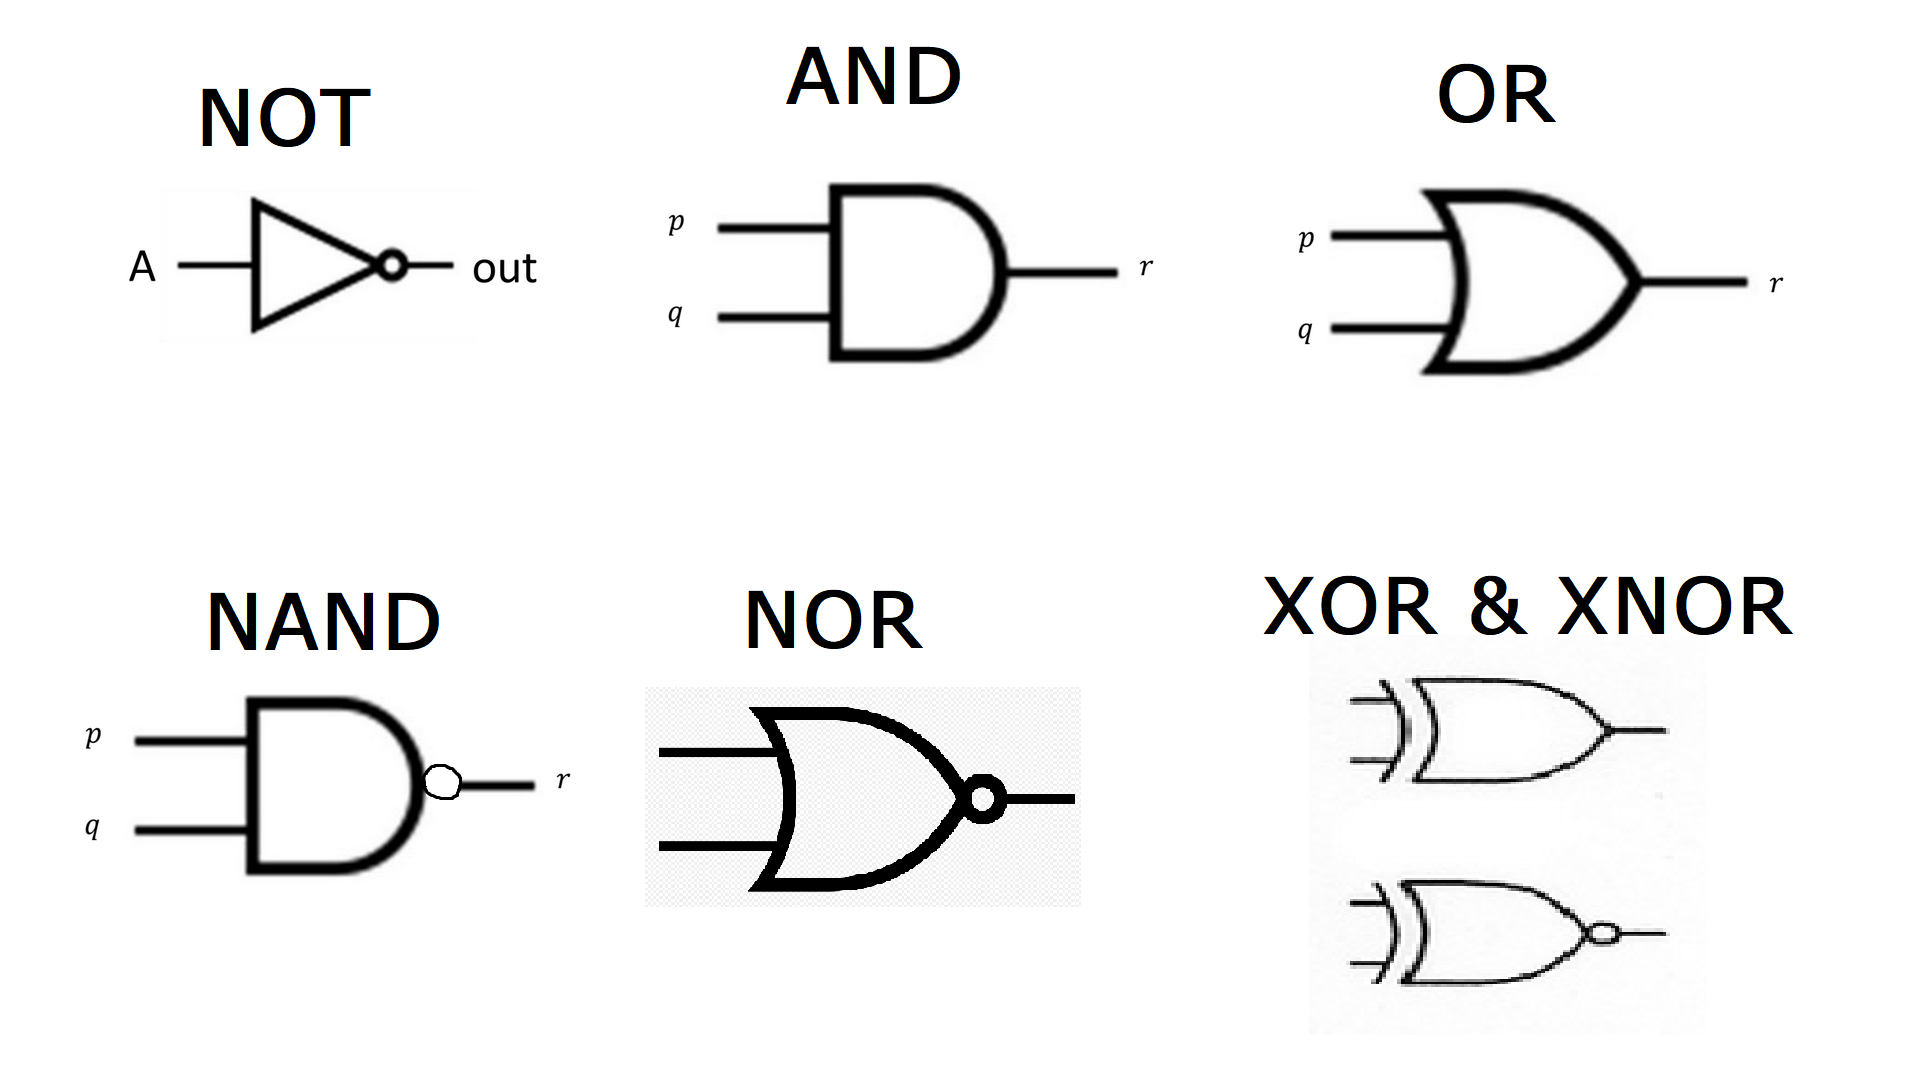
\includegraphics[width=\textwidth]{Ch2/circuit_ops.png}
    \caption{Circuit diagram gates}
    \label{fig:circ}
\end{figure}

The following question is a review from Thursday's lecture.

\begin{enumerate}
    \item Write $x \oplus y$ (XOR) using only the and ($\land$), or ($\lor$), and not ($\shortsim$) operations.
    \item Construct a circuit representing the boolean formula you wrote in part a).
\end{enumerate}